\documentclass[hyperref={pdfpagelabels=false}]{beamer}
% Die Hyperref Option hyperref={pdfpagelabels=false} verhindert die Warnung:
% Package hyperref Warning: Option `pdfpagelabels' is turned off
% (hyperref)                because \thepage is undefined. 
% Hyperref stopped early 
%
\usepackage{hyperref}
\usepackage{lmodern}
% Das Paket lmodern erspart die folgenden Warnungen:
% LaTeX Font Warning: Font shape `OT1/cmss/m/n' in size <4> not available
% (Font)              size <5> substituted on input line 22.
% LaTeX Font Warning: Size substitutions with differences
% (Font)              up to 1.0pt have occurred.
%

\graphicspath{{./Bilder/}}
\usepackage[ngerman]{babel}
\usepackage{amssymb}
\usepackage[utf8]{inputenc}


% Wenn \titel{\ldots} \author{\ldots} erst nach \begin{document} kommen,
% kommt folgende Warnung:
% Package hyperref Warning: Option `pdfauthor' has already been used,
% (hyperref) ... 
% Daher steht es hier vor \begin{document}

\title{Automatisierte Analyse von Preisbildungsmustern anhand von Zeitreihendaten der Markttransparenzstelle für Kraftstoffe}   
\author{Kai Fritsch} 
\date{\today} 

% zusaetzlich ist das usepackage{beamerthemeshadow} eingebunden 
\usepackage{beamerthemeshadow}

%  \beamersetuncovermixins{\opaqueness<1>{25}}{\opaqueness<2->{15}}
%  sorgt dafuer das die Elemente die erst noch (zukuenftig) kommen 
%  nur schwach angedeutet erscheinen 
\beamersetuncovermixins{\opaqueness<1>{25}}{\opaqueness<2->{15}}
% klappt auch bei Tabellen, wenn teTeX verwendet wird\ldots
\begin{document}


\begin{frame}
\titlepage
\end{frame} 

\section{Einleitung \& Zielsetzung} 
\begin{frame}
\frametitle{Hintergrundinformationen} 
\begin{itemize}
\item Einführung Markttransparenzstelle für Kraftstoffe
\item Verfügbarkeit aller aktuellen Preise in Echtzeit
\item Verstärktes Konkurrenzverhalten
\item Hochfrequente Preisänderungen
\end{itemize} 
\end{frame}

\begin{frame}
\frametitle{Erster Einblick} 
\href{http://10.1.0.1:8091/client/}{Tankstellenkarte}
\end{frame}

\begin{frame}
\frametitle{Automatisierung} 
\begin{itemize}
\item Konkurrenten bestimmen
\end{itemize}
\end{frame}

\begin{frame}
\frametitle{Konkurrenten bestimmen}
\begin{center}
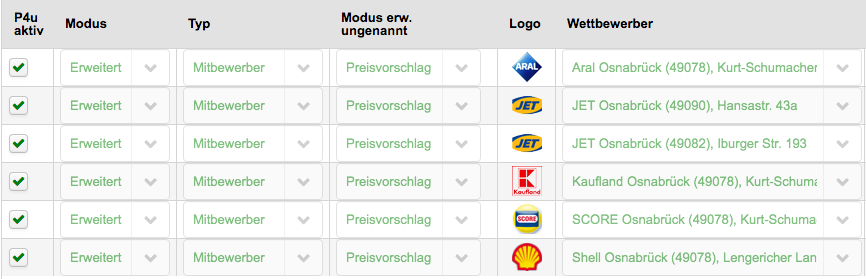
\includegraphics[scale=0.35]{konkurenz.png}
\end{center}
\end{frame}

\begin{frame}
\frametitle{Automatisierung}
\begin{itemize}
\item Konkurrenten bestimmen
\item Regeln festlegen
\end{itemize}
\end{frame}

\begin{frame}
\frametitle{Regeln festlegen}
\begin{center}
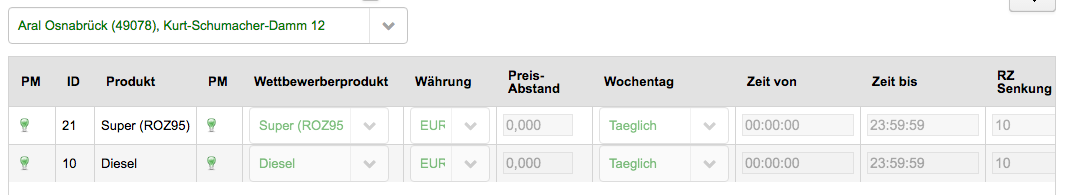
\includegraphics[scale=0.30]{regeln1.png}
\end{center}
\end{frame}

\begin{frame}
\frametitle{Automatisierung}
\begin{itemize}
\item Konkurrenten bestimmen
\item Regeln festlegen
\item Automatisierung wählen
\end{itemize}
\end{frame}

\begin{frame}
\frametitle{Automatisierung wählen}
\begin{center}
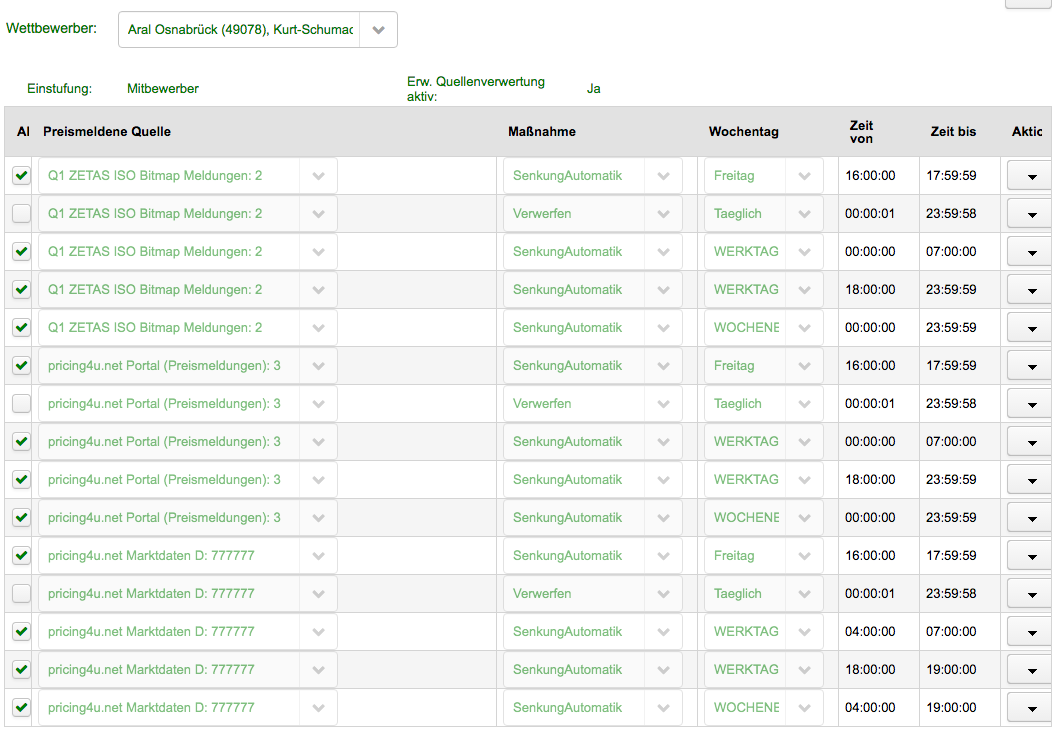
\includegraphics[scale=0.2]{automatik.png}
\end{center}
\end{frame}

\begin{frame}
\frametitle{Genauere Analyse} 
\href{http://10.1.0.1:8091/client/}{Tankstellenkarte}
\end{frame}

\section{Umsetzung der Regelerkennung}

\begin{frame}
\frametitle{Vorauswahl an Konkurrenten treffen}
\begin{itemize}
\item Vekehrsfluss ist schwer automatisch bestimmbar
\item Abstand spielt eine wichtige Rolle
\item Besiedelungsdichte hat einen starken Einfluss auf den Abstand
\end{itemize}
\end{frame}

\begin{frame}
\frametitle{Ansatz Konkurrenz erkennen}
\begin{itemize}
\item Differenz-Zeitreihen analysieren
\item Brute force alle Regeln probieren 
\item Zeitaufwändig und an einigen stellen Problematisch
\item Preisänderungen sind die interessanten Zeitpunkte
\end{itemize}
\end{frame}

\begin{frame}
\frametitle{Reaktionen erkennen}
\begin{itemize}
\item Zeitabstand von Aktion und Reaktion
\item Reaktionshöhe von Aktion und Reaktion
\end{itemize}
\end{frame}

\begin{frame}
\frametitle{Reaktionen erkennen}
\begin{center}
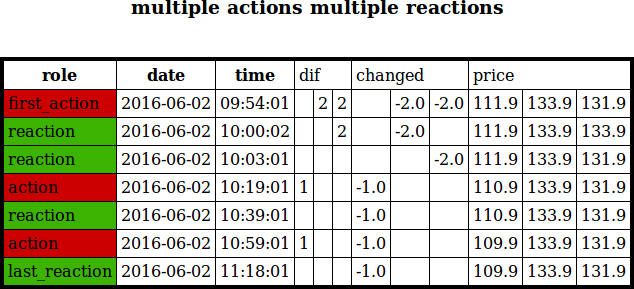
\includegraphics[scale=0.30]{mamr.jpg}
\end{center}
\end{frame}

\begin{frame}
\frametitle{Reaktionen erkennen}
\begin{center}
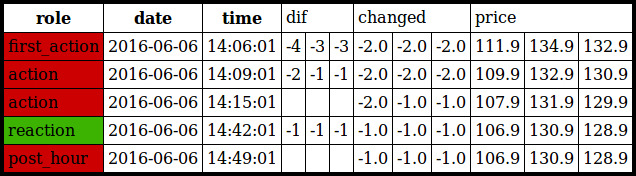
\includegraphics[scale=0.30]{masr.jpg}
\end{center}
\end{frame}

\begin{frame}
\frametitle{Reaktionen erkennen}
\begin{center}
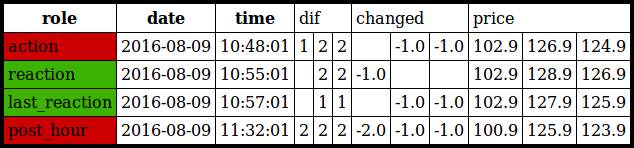
\includegraphics[scale=0.30]{samr2.jpg}
\end{center}
\end{frame}

\begin{frame}
\frametitle{Reaktionen erkennen}
\begin{itemize}
\item Zeitabstand von Aktion und Reaktion
\item Reaktionshöhe von Aktion und Reaktion
\item Logik zur Erkennung der tatsächlichen Reaktionen
\end{itemize}
\end{frame}

\begin{frame}
\frametitle{Regeln bestimmen}
\begin{itemize}
\item Potentielle Reaktionen bestehen zu fast jeder Tankstelle
\item Genauso wichtig sind nicht erfolgte Reaktionen
\item Der maximale Abstand nach ignorierten Änderungen oder Reaktionen ist ausschlaggebend
\item Ausreißer sind möglich
\end{itemize}
\end{frame}

\begin{frame}
\frametitle{Zeitintervall festlegen}
\begin{itemize}
\item Öffnungszeiten müssen berücksichtigt werden
\item Mindestanzahl an Daten pro Zeitintervall werden benötigt
\item Starke Schwankungen zwischen verschiedenen Intervallen berücksichtigen
\item Ausreißer sind möglich
\end{itemize}
\end{frame}

\section{Auswertung \& Fazit}
\begin{frame}
\frametitle{Visualisierung Ergebnisse} 
\href{http://10.1.0.1:8091/client/}{Tankstellenkarte}
\end{frame}


\end{document}
